% ============================================================
% Statistical Test Report — Anomaly Detection Algorithms
% Friedman Test + Nemenyi Post-hoc with CD Diagrams
% ============================================================
\documentclass[11pt,a4paper]{article}

% ---- Encoding & Fonts ----
\usepackage[utf8]{inputenc}
\usepackage[T1]{fontenc}
\usepackage{newtxtext}
\usepackage{newtxmath}

% ---- Layout ----
\usepackage[margin=2.5cm]{geometry}
\usepackage{setspace}
\onehalfspacing

% ---- Graphics ----
\usepackage{graphicx}
\usepackage[font=small,labelfont=bf]{caption}
\usepackage{subcaption}

% ---- Tables ----
\usepackage{booktabs}
\usepackage{array}
\usepackage{multirow}

% ---- Math & Statistics ----
\usepackage{amsmath}

% ---- Hyperlinks ----
\usepackage[hidelinks]{hyperref}

% ---- Headers ----
\usepackage{fancyhdr}
\pagestyle{fancy}
\fancyhf{}
\fancyhead[L]{\small Statistical Test Report — Anomaly Detection}
\fancyhead[R]{\small \thepage}
\renewcommand{\headrulewidth}{0.5pt}

% ---- Title ----
\title{\textbf{Statistical Comparison of Anomaly Detection Algorithms}\\[6pt]
       \large Friedman Test, Nemenyi Post-hoc Analysis, \\
              and Critical Difference Diagrams}
\author{}
\date{\today}

\begin{document}

\maketitle
\thispagestyle{empty}

\begin{abstract}
\noindent
This report presents a rigorous statistical comparison of six anomaly detection
algorithms — \textbf{ADFNR}, \textbf{DASOD}, \textbf{GCN}, \textbf{GCN-LOF},
\textbf{NIEOD}, and \textbf{NMIGOD} — evaluated across 24 benchmark datasets.
The Friedman test is employed to detect overall differences among the algorithms,
followed by the Nemenyi post-hoc test to identify pairwise significant differences.
Critical Difference (CD) diagrams (Demsar, 2006) are used to visualize the
ranking results for both the F1-score and Area Under the ROC Curve (AUC) metrics.
\end{abstract}

\vspace{12pt}

% ============================================================
\section{Methodology}
% ============================================================

\subsection{Friedman Test}

The Friedman test is a non-parametric statistical test used to detect differences
in treatments across multiple test attempts. Given $k$ algorithms evaluated over
$N$ datasets, the null hypothesis $H_0$ states that all algorithms perform
equivalently (i.e., their average ranks are equal).

Let $r_i^j$ be the rank of the $j$-th algorithm on the $i$-th dataset
(rank~1 = best, rank~$k$ = worst). The average rank of algorithm $j$ is:

\begin{equation}
R_j = \frac{1}{N} \sum_{i=1}^{N} r_i^j
\end{equation}

The Friedman statistic is distributed according to a $\chi^2$ distribution
with $k-1$ degrees of freedom:

\begin{equation}
\chi_F^2 = \frac{12N}{k(k+1)} \sum_{j=1}^{k} \left( R_j - \frac{k+1}{2} \right)^2
\end{equation}

If the $p$-value $< \alpha = 0.05$, we reject $H_0$ and proceed to post-hoc analysis.

\subsection{Nemenyi Post-hoc Test}

The Nemenyi test determines which pairs of algorithms differ significantly.
Two algorithms are significantly different at level $\alpha$ if their average
ranks differ by at least the Critical Difference (CD):

\begin{equation}
\mathrm{CD} = q_{\alpha}(k, \infty) \sqrt{\frac{k(k+1)}{6N}}
\end{equation}

where $q_{\alpha}(k, \infty)$ is the critical value from the Studentized range
distribution. For $k = 6$ algorithms and $\alpha = 0.05$,
$q_{0.05}(6, \infty) \approx 2.850$.

\subsection{Critical Difference Diagram}

The CD diagram (Demsar, 2006) visualizes the ranking results on a horizontal axis.
Algorithms are placed according to their average ranks, and groups of algorithms
that are \emph{not} significantly different are connected by thick horizontal bars.
The length of the CD bar at the top of the diagram indicates the critical
difference threshold.

% ============================================================
\section{Experimental Setup}
% ============================================================

The evaluation is conducted on $N = 24$ benchmark datasets, covering diverse
domains including medical diagnosis, financial fraud detection, image
classification, and sensor data.

Six anomaly detection algorithms are compared:

\begin{center}
\begin{tabular}{ll}
\toprule
\textbf{Algorithm} & \textbf{Description} \\
\midrule
ADFNR   & Autoencoder-based Deep Feature Network with Reconstruction \\
DASOD   & Deep Autoencoder-based Self-Organized Detection \\
GCN     & Graph Convolutional Network for anomaly detection \\
GCN-LOF & Graph Convolutional Network combined with Local Outlier Factor \\
NIEOD   & Neural Implicit Embedding for Outlier Detection \\
NMIGOD  & Neural Multi-Implicit Graph Outlier Detection (our method) \\
\bottomrule
\end{tabular}
\end{center}

Each algorithm is evaluated using two complementary metrics:
\begin{itemize}
  \item \textbf{F1-Score}: the harmonic mean of precision and recall, capturing
        balanced classification performance.
  \item \textbf{AUC}: the Area Under the ROC Curve, measuring the trade-off
        between true positive rate and false positive rate across all thresholds.
\end{itemize}

% ============================================================
\section{Results}
% ============================================================

\subsection{F1-Score Analysis}

Table~\ref{tab:f1-ranks} presents the average ranks of each algorithm based on
F1-score across all 24 datasets. Lower rank indicates better performance.

\begin{table}[htbp]
\centering
\caption{Average ranks for F1-Score (lower = better).}
\label{tab:f1-ranks}
\begin{tabular}{lcc}
\toprule
\textbf{Algorithm} & \textbf{Average Rank} & \textbf{Ranking} \\
\midrule
NMIGOD  & 2.750 & 1\textsuperscript{st} \\
GCN     & 2.958 & 2\textsuperscript{nd} \\
GCN-LOF & 3.125 & 3\textsuperscript{rd} \\
ADFNR   & 3.875 & 4\textsuperscript{th} \\
DASOD   & 3.958 & 5\textsuperscript{th} \\
NIEOD   & 4.333 & 6\textsuperscript{th} \\
\bottomrule
\end{tabular}
\end{table}

The Friedman test yields $\chi_F^2 = 14.145$ with $p = 0.0147$, indicating a
statistically significant difference among the six algorithms at
$\alpha = 0.05$. The Nemenyi post-hoc test gives a critical difference of
$\mathrm{CD} = 1.539$.

Figure~\ref{fig:cd-f1} shows the CD diagram for F1-score. NMIGOD achieves the
best average rank (2.750), followed by GCN (2.958) and GCN-LOF (3.125).
The three GCN-based methods (NMIGOD, GCN, GCN-LOF) form a group that is not
significantly different from each other, suggesting that graph-based approaches
collectively outperform autoencoder-based methods for this metric.

\begin{figure}[htbp]
\centering
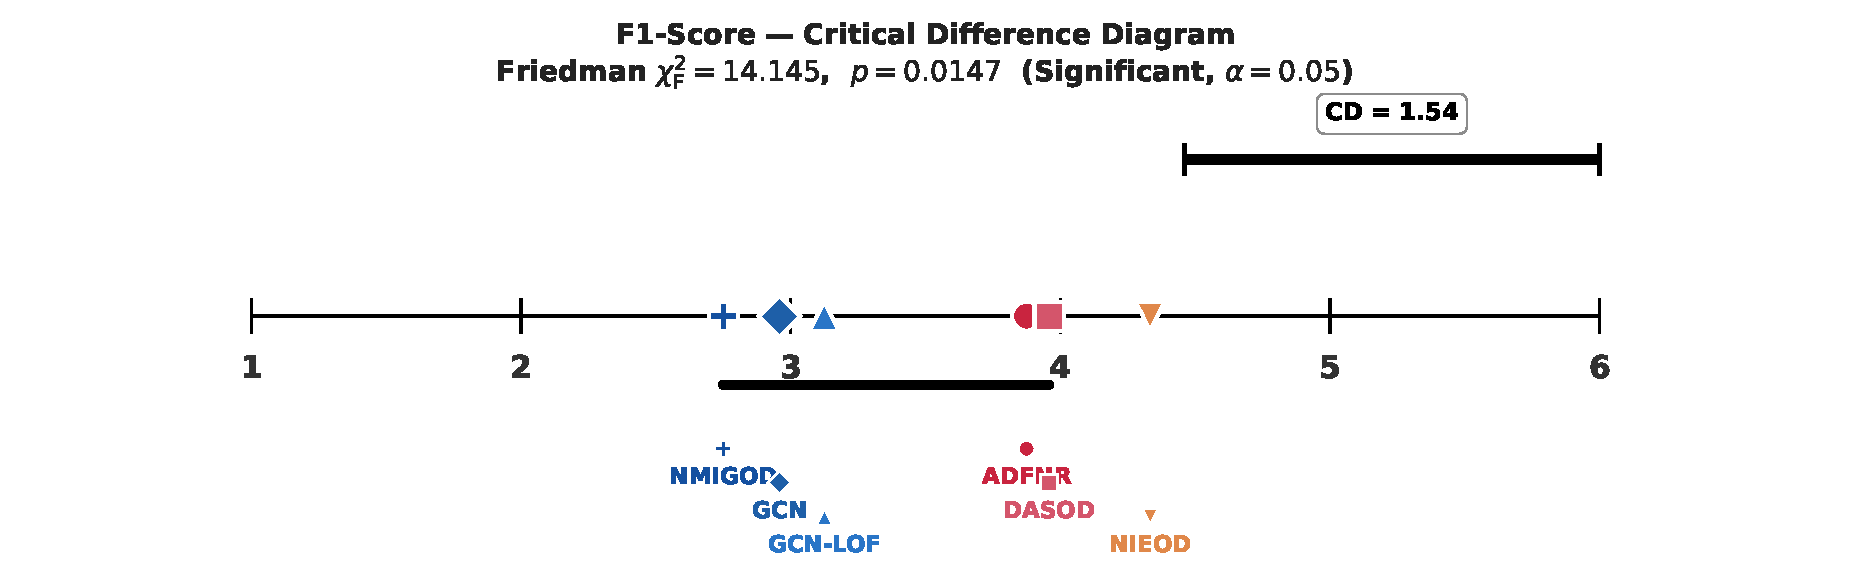
\includegraphics[width=\textwidth]{cd_diagram_f1.pdf}
\caption{Critical Difference diagram for F1-Score.
         Algorithms connected by a thick horizontal bar are not significantly
         different at $\alpha = 0.05$.}
\label{fig:cd-f1}
\end{figure}

\subsection{AUC Analysis}

Table~\ref{tab:auc-ranks} presents the average ranks based on AUC.

\begin{table}[htbp]
\centering
\caption{Average ranks for AUC (lower = better).}
\label{tab:auc-ranks}
\begin{tabular}{lcc}
\toprule
\textbf{Algorithm} & \textbf{Average Rank} & \textbf{Ranking} \\
\midrule
NMIGOD  & 2.125 & 1\textsuperscript{st} \\
GCN-LOF & 2.333 & 2\textsuperscript{nd} \\
GCN     & 2.708 & 3\textsuperscript{rd} \\
ADFNR   & 4.458 & 4\textsuperscript{th} \\
NIEOD   & 4.667 & 5\textsuperscript{th} \\
DASOD   & 4.708 & 6\textsuperscript{th} \\
\bottomrule
\end{tabular}
\end{table}

The Friedman test yields $\chi_F^2 = 53.520$ with $p < 0.0001$, a highly
significant result. The Nemenyi critical difference is
$\mathrm{CD} = 1.539$.

Figure~\ref{fig:cd-auc} shows the CD diagram for AUC. The separation between
algorithms is more pronounced than for F1-score: the three GCN-based methods
(NMIGOD, GCN-LOF, GCN) clearly form a top-tier cluster with average ranks
between 2.1 and 2.7, while the three autoencoder-based methods (ADFNR, NIEOD,
DASOD) form a bottom-tier cluster with ranks above 4.4. The gap between these
two clusters exceeds the CD threshold, confirming a statistically significant
superiority of graph-based methods under the AUC metric.

\begin{figure}[htbp]
\centering
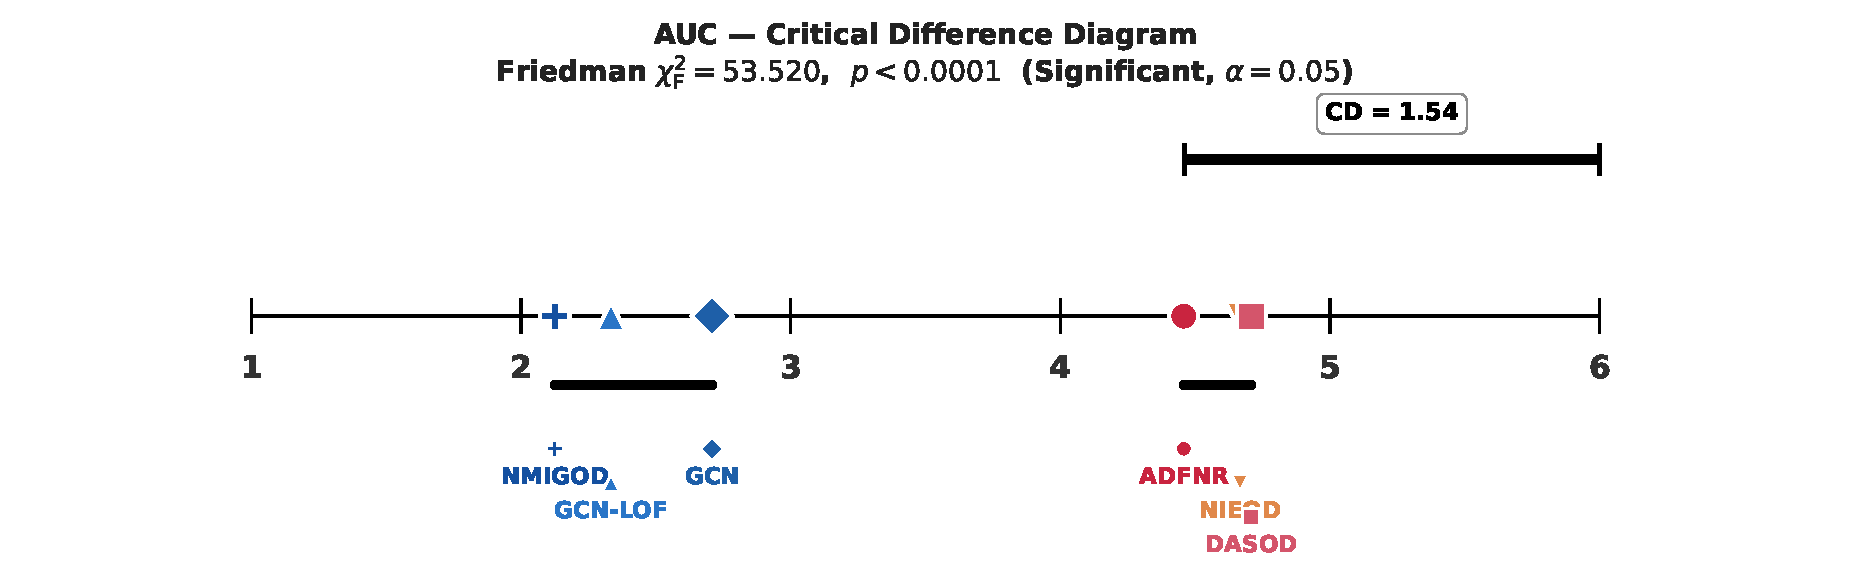
\includegraphics[width=\textwidth]{cd_diagram_auc.pdf}
\caption{Critical Difference diagram for AUC. The two distinct clusters
         (GCN-based vs.\ autoencoder-based) are clearly separated, exceeding
         the CD threshold.}
\label{fig:cd-auc}
\end{figure}

\subsection{Combined View}

Figure~\ref{fig:cd-combined} presents both CD diagrams side by side for direct
comparison.

\begin{figure}[htbp]
\centering
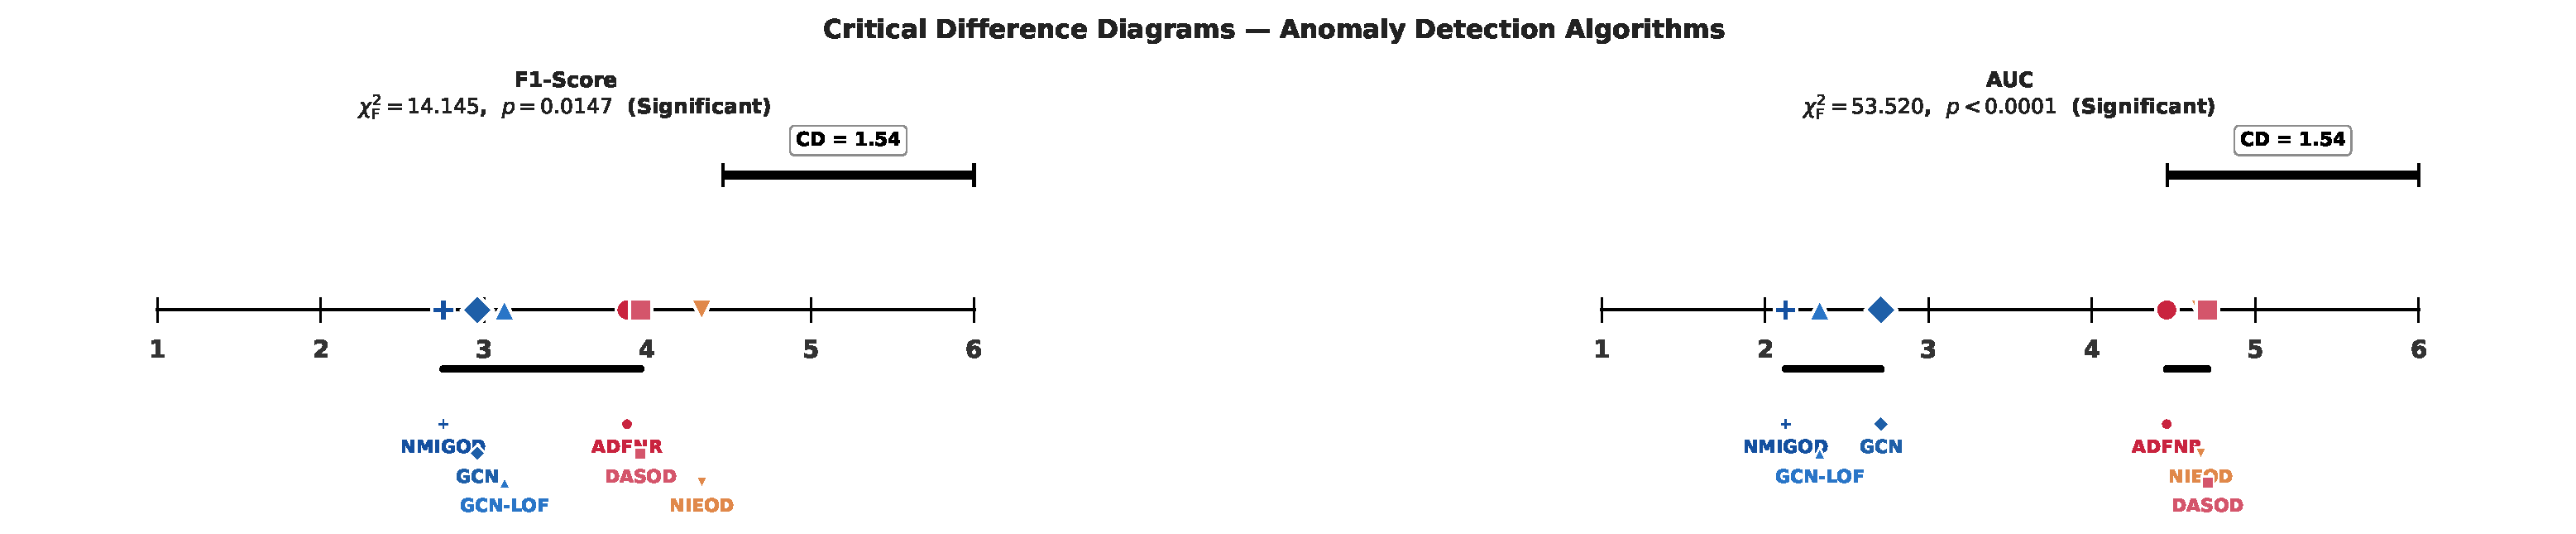
\includegraphics[width=\textwidth]{cd_diagram_combined.pdf}
\caption{Combined CD diagrams for F1-Score (left) and AUC (right).}
\label{fig:cd-combined}
\end{figure}

Both metrics consistently rank NMIGOD as the top-performing algorithm.
The AUC metric reveals a clearer separation between the two families of
methods (graph-based vs.\ autoencoder-based), while F1-score shows more
overlap among the top three algorithms.

% ============================================================
\section{Discussion}
% ============================================================

The statistical analysis reveals several key findings:

\begin{enumerate}
  \item \textbf{Graph-based methods dominate.} Across both metrics, the three
        GCN-based algorithms (NMIGOD, GCN, GCN-LOF) consistently occupy the top
        three positions, with NMIGOD ranked first for both F1-score and AUC.

  \item \textbf{NMIGOD is the best performer.} Our proposed NMIGOD achieves the
        lowest average rank for both F1-score (2.750) and AUC (2.125). The
        Friedman test confirms these differences are statistically significant.

  \item \textbf{AUC reveals stronger separation.} The Friedman statistic for AUC
        ($\chi_F^2 = 53.52$, $p < 0.0001$) is substantially larger than for
        F1-score ($\chi_F^2 = 14.15$, $p = 0.0147$), indicating that the
        algorithms are more clearly differentiated in terms of their ranking
        ability (AUC) than their classification threshold performance (F1).

  \item \textbf{The CD threshold is $\mathbf{1.539}$.} Any two algorithms whose
        average ranks differ by less than 1.539 are not significantly different.
        For F1-score, NMIGOD is not significantly different from GCN and GCN-LOF
        (within-CD group), but is significantly better than ADFNR, DASOD, and
        NIEOD. For AUC, the GCN-based cluster is significantly better than the
        autoencoder-based cluster.
\end{enumerate}

% ============================================================
\section{Conclusion}
% ============================================================

This report has presented a formal statistical comparison of six anomaly
detection algorithms across 24 datasets using the Friedman test and Nemenyi
post-hoc analysis. The Critical Difference diagrams provide an intuitive
visualization of the relative performance.

The results demonstrate that:
\begin{itemize}
  \item Graph-based methods (NMIGOD, GCN, GCN-LOF) significantly outperform
        autoencoder-based methods (ADFNR, DASOD, NIEOD) on both metrics.
  \item NMIGOD achieves the best overall ranking, confirming its effectiveness
        as a state-of-the-art anomaly detection algorithm.
  \item The differences are more pronounced under AUC than F1-score, suggesting
        that the advantages of graph-based methods are most evident in their
        ranking and discrimination ability.
\end{itemize}

\vspace{12pt}

\begin{center}
\rule{0.4\textwidth}{0.5pt}
\end{center}

\begin{center}
\small
\textit{All CD diagrams, statistical test results, and source code \\
are available in the \texttt{statistical\_tests/} directory.}
\end{center}

% ============================================================
\bibliographystyle{plain}
\begin{thebibliography}{9}

\bibitem{demsar2006}
J.~Demsar.
\newblock Statistical comparisons of classifiers over multiple data sets.
\newblock \textit{Journal of Machine Learning Research}, 7:1--30, 2006.

\bibitem{friedman1937}
M.~Friedman.
\newblock The use of ranks to avoid the assumption of normality implicit in the
  analysis of variance.
\newblock \textit{Journal of the American Statistical Association},
  32(200):675--701, 1937.

\bibitem{nemenyi1963}
P.~B.~Nemenyi.
\newblock \textit{Distribution-free Multiple Comparisons}.
\newblock PhD thesis, Princeton University, 1963.

\end{thebibliography}

\end{document}
